% !TEX root = ../main.tex
% Appendix A source fragment. Do not input this file into the six-page paper.
% The overall portfolio wrapper must load booktabs and pdfpages, create the
% Appendix A title page, establish A.1/A.2/... pagination and define the
% optional imported-page hook below.
\providecommand{\PortfolioImportedPageCommand}{}

\phantomsection
\addcontentsline{toc}{subsection}{A.1 Summary of GenAI Use}
\subsection*{A.1 Summary of GenAI Use}
\label{app:a-summary}

Generative artificial intelligence (GenAI) tools were used as drafting and
documentation aids during the project. They did not generate the simulation
dataset or replace the reported model training and evaluation. Table~
\ref{tab:appendix-a-summary} identifies the use recorded in the current
cumulative log, its benefit and the parts of the project that it informed.

\begin{table}[htbp]
    \caption{GenAI use recorded in the current cumulative log.}
    \label{tab:appendix-a-summary}
    \centering
    \scriptsize
    \begin{tabular}{@{}p{0.14\textwidth}p{0.25\textwidth}
                         p{0.25\textwidth}p{0.25\textwidth}@{}}
        \toprule
        Tool and period & Purpose and benefit & Material informed
          & Review and limitations \\
        \midrule
        Claude Code,
        Weeks 7--10
          & Summarised Git history and helped organise development-log
            material, saving time when tracing changes across files and
            commits.
          & Bi-weekly development records later consulted when preparing the
            progress and milestone account in Appendix C.
          & The summaries were checked against commits and project files.
            Work outside version control and experimental quality still
            required manual review. \\
        Gemini,
        Week 11--12
          & Drafted a progress summary and helped interpret milestone status
            consistently.
          & The Week 11--12 development record and the progress/status account
            consolidated in Appendix C.
          & Dates, milestones and implementation claims were checked against
            the repository and approved project plan. \\
        Gemini Notebook
        (NotebookLM),
        Week 13--14
          & Condensed the project narrative, organised prior work into themes
            and produced an initial LaTeX design-variable table.
          & The paper's Abstract, Introduction, Prior Work discussion and
            Table I in Section III.
          & Claims were checked against primary papers, executed notebooks and
            saved metrics. Unsupported statements, including claims that
            passivity and causality were enforced, were corrected. \\
        \bottomrule
    \end{tabular}
\end{table}

The tools were used to propose summaries, structure and wording. Experimental
values in the paper and appendices were taken from executed notebooks and saved
artifacts, then independently reproduced in Notebook 07. Literature claims were
checked against the cited sources. Generated text was revised for accuracy,
scope and consistency with the completed work. The author remains responsible
for the final content.

\clearpage
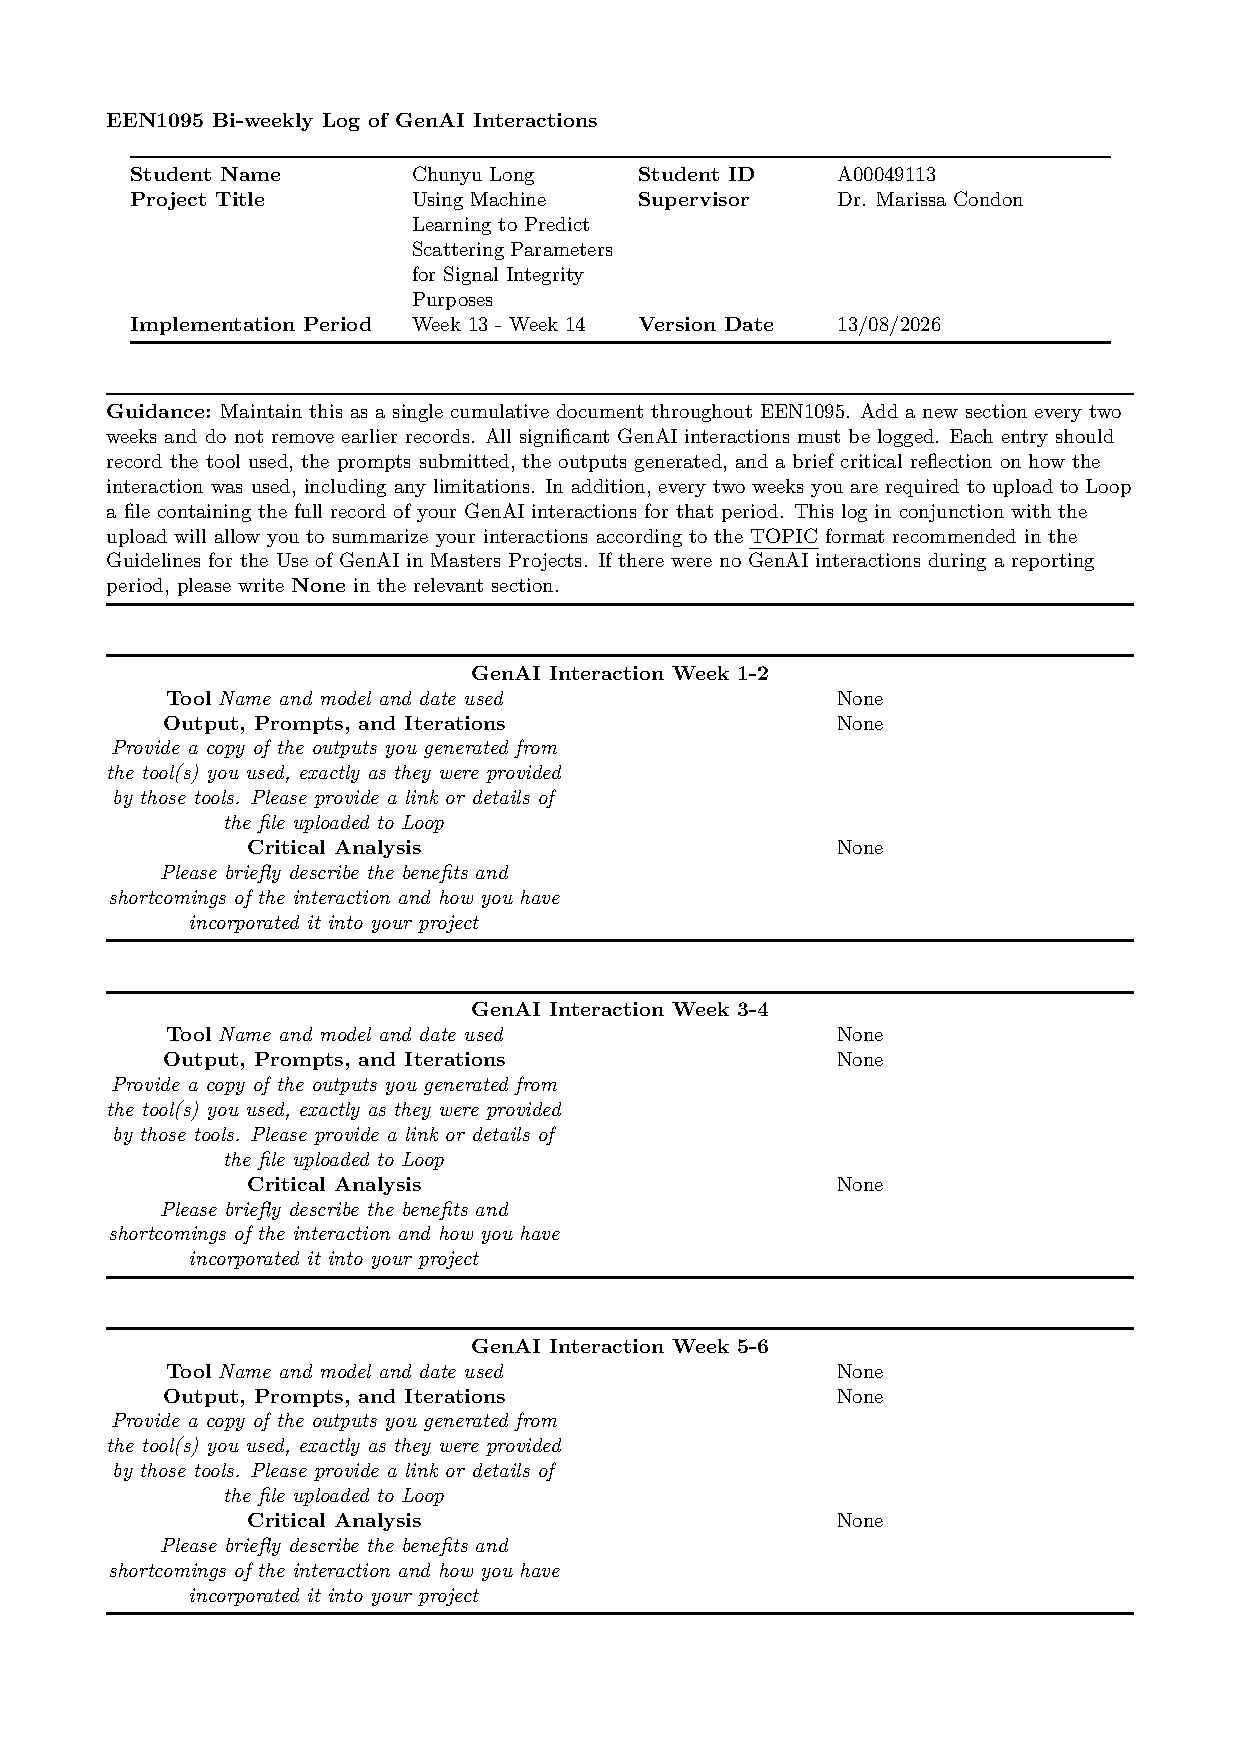
\includepdf[
    pages=-,
    fitpaper=true,
    pagecommand={\PortfolioImportedPageCommand},
    addtotoc={1,subsection,2,{A.2 Cumulative Bi-weekly GenAI Log},
              app:a-cumulative-log}
]{documents/EEN1095_Biweekly_GenAI_Log.pdf}
